% --------------------------------------------------------------------------------------------------
% Section: Clinical Manifestations
% Describes how lung cancer presents symptomatically, including early and advanced signs of disease.
% --------------------------------------------------------------------------------------------------

\section{Clinical Manifestations}

% Introductory paragraph explaining the typical timing and variability of lung cancer symptoms.
Lung cancer often does not cause symptoms in its early stages. Most clinical manifestations appear 
as the disease progresses, and they can vary depending on the location and extent of the tumor, as 
well as whether the cancer has spread (metastasized) to other parts of the body.

% --------------------------------------------------------------------------------------------------
% Subsection: Early Warning Signs
% Describes the nonspecific symptoms that may help identify lung cancer early, before metastasis.
% --------------------------------------------------------------------------------------------------

\subsection{Early Warning Signs}

% Explanation that early detection is possible despite nonspecific presentation; persistent symptoms
% are key.
Early warning signs can occur, and recognizing these symptoms can lead to earlier diagnosis and 
improved outcomes. Many of these symptoms are nonspecific and can be mistaken for other, less 
serious conditions, so persistence or worsening of these symptoms warrants medical evaluation.

% Figure: Visual representation of frequency/distribution of early symptoms.

\vspace{1em}
\begin{center}
    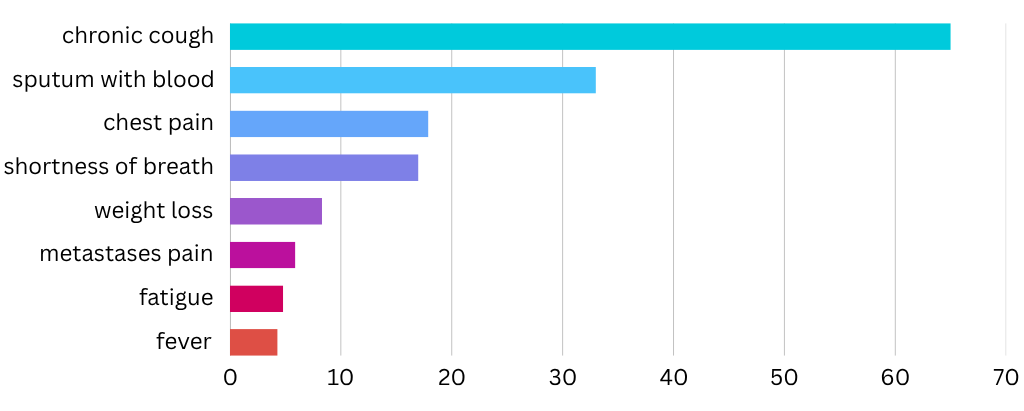
\includegraphics[width=\textwidth]{../assets/03-clinical/early-signs.png}  

    \small\textit{Distribution of early symptoms. Data source: \cite{cm2019}}
\end{center}
\vspace{1em}

% Itemized bullet list for clarity: early signs broken into 3 tiers - common, very common, less 
% common.
\begin{itemize}
    % Most typical initial presentations
    \item \textbf{Common early signs:}
        \begin{itemize}
            \item \textbf{Persistent Cough:} A new cough that does not go away after three weeks, 
            or a long-standing cough that worsens, is one of the most frequent early signs.

            \item \textbf{Coughing Up Blood:} Even small amounts of blood or rust-colored sputum 
            can be an early warning sign and should be evaluated promptly.
    
            \item \textbf{Chest or Shoulder Pain:} Unexplained pain or discomfort in the chest or 
            shoulder, especially if it worsens with breathing, coughing, or laughing.
        
            \item \textbf{Wheezing:} A new onset of wheezing or a whistling sound when breathing, 
            not previously experienced, may indicate airway obstruction.
        \end{itemize}
    
    % These occur early and are especially indicative when combined with other signs
    \newpage
    \item \textbf{Very common early signs}:
        \begin{itemize}
            \item \textbf{Unexplained Weight Loss:} Losing weight without trying, especially if 
            significant.

            \item \textbf{Loss of Appetite:} A decrease in appetite not attributable to other 
            causes.
    
            \item \textbf{Fatigue:} Feeling unusually tired or lacking energy, even with adequate 
            rest.
        \end{itemize}
    
    % These are rarer but strongly associated with malignancy when present.
    \item \textbf{Less common early signs}:
        \begin{itemize}
            \item \textbf{Swelling of Face or Neck:} Can occur if a tumor obstructs blood flow in 
            the chest.

            \item \textbf{Finger Clubbing:} Changes in the shape of the fingertips, such as 
            becoming more curved or enlarged, known as clubbing.
        \end{itemize}
\end{itemize}

% --------------------------------------------------------------------------------------------------
% Subsection: Progressed Stage Symptoms
% Describes signs and symptoms in advanced lung cancer (Stage 3-4), including systemic effects.
% --------------------------------------------------------------------------------------------------

\subsection{Progressed Stage Symptoms}

% General explanation of disease severity, staging, prognosis, and diagnosis trends.
As lung cancer advances to later stages (Stage 3 and Stage 4), symptoms become more pronounced, 
severe, and diverse due to tumor growth, local invasion, and metastasis to other organs. These 
progressed stage symptoms reflect both the direct effects of the tumor in the lungs and systemic 
manifestations related to cancer spread. Unfortunately, over half of lung cancer cases (52\%) are 
diagnosed at the distant metastatic stage, which is associated with poor prognosis and only about 
23\% of cases are diagnosed at an early localized stage, where curative treatments are more 
effective and survival rates are significantly higher.

% Figure: Bar or pie chart showing lung cancer diagnosis by stage (visualizing late vs. early 
% detection).
\vspace{1em}
\begin{center}
    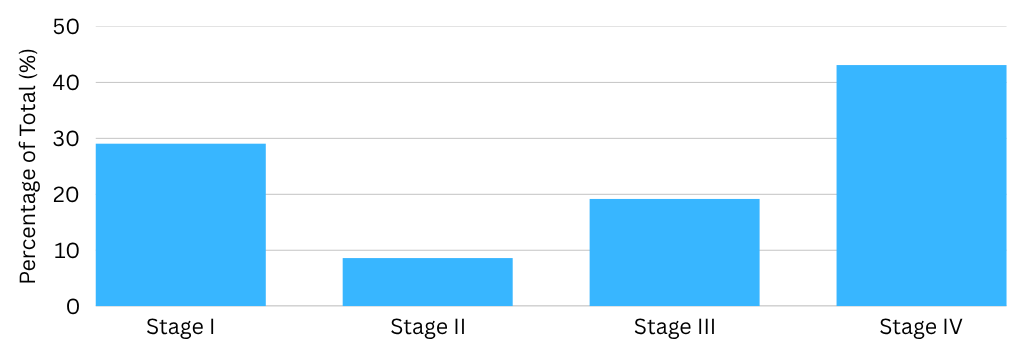
\includegraphics[width=\textwidth]{../assets/03-clinical/stages-diagnosis.png}  

    \textit{Lung cancer diagnoses by stage (2010--2017). Data source: \cite{jco2022}}
\end{center}
\vspace{1em}

\newpage
\begin{itemize}
    % Local effects of advanced tumor burden
    \item \textbf{Common Symptoms in Progressed Lung Cancer Stages (Stage 3 and 4):}
        \begin{itemize}
            \item \textit{Shortness of Breath (Dyspnea):} Increasing difficulty breathing due to 
            airway obstruction, tumor growth, or pleural effusion (fluid accumulation around the 
            lungs).

            \item \textit{Hoarseness:} Caused by tumor involvement of the recurrent laryngeal nerve, 
            leading to voice changes.

            \item \textit{Frequent Lung Infections:} Recurrent or persistent infections such as 
            bronchitis or pneumonia due to impaired lung function and obstruction.
        \end{itemize}
    
    % Signs and symptoms of metastatic spread to distant organs
    \item \textbf{Symptoms Related to Tumor Spread (Metastasis):}
        \begin{itemize}
            \item \textit{Lymph Node Enlargement:} Swelling of lymph nodes near the collarbone, 
            neck, or elsewhere.

            \item \textit{Neurological Symptoms:} Headaches, dizziness, seizures, memory problems, 
            mood or personality changes, numbness, or balance issues due to brain metastases.

            \item \textit{Jaundice:} Yellowing of the skin and eyes from liver metastases.

            \item \textit{Horner Syndrome:} Drooping eyelid, small pupil, and decreased sweating on 
            one side of the face due to tumor involvement of sympathetic nerves.
        \end{itemize}
    
    % Systemic metabolic/hormonal effects from secretions by tumors
    \item \textbf{Paraneoplastic Syndromes:}
    In progressed lung cancer, tumors may produce hormones or hormone-like substances causing 
    systemic effects known as paraneoplastic syndromes: muscle weakness, nausea and vomiting, high 
    blood pressure, high blood sugar, confusion and seizures.  
\end{itemize}
